%\setcounter{section}{27}
\section{CÔNG THỨC CỘNG XÁC SUẤT}
\subsection{LÝ THUYẾT CẦN NHỚ}
\subsubsection{PHÉP TOÁN TRÊN CÁC BIẾN CỐ}
Cho hai biến cố $A$ và $B$. Khi đó $A, B$ là các tập con của không gian mẫu $\Omega$.
\begin{enumerate}[\iconMT]
	\immini{\item \indam{Biến cố hợp:} Biến cố: \lq\lq $A$ hoặc $B$ xảy ra\rq\rq\ được gọi là biến cố hợp của $A$ và $B$.
		\begin{itemize}
			\item  [$\bullet$] Kí hiệu là $A \cup B$.
			\item  [$\bullet$] Biến cố hợp $A \cup B$ là tập con của không gian mẫu $\Omega$.
		\end{itemize}
	}{
\begin{tikzpicture}[scale=1,rotate=5]
	\def\firstcircle{(0:0) ellipse (1.2 cm and 1 cm)}
	\def\secondcircle{(0:1.8) ellipse (1 cm and 1 cm)}
	\fill[pattern=north east lines] \firstcircle;
	\fill[pattern=north east lines] \secondcircle;
	\draw \firstcircle node[fill=white,left]{$A$};
	\draw \secondcircle node [fill=white,right=-0.1]{$B$};
\end{tikzpicture}}
	\immini{\item \indam{Biến cố giao:} Biến cố: \lq\lq Cả $A$ và $B$ đều xảy ra\rq\rq\ được gọi là biến cố giao của $A$ và $B$.
		\begin{itemize}
			\item [$\bullet$] Kí hiệu là $A \cap B$ hoặc $A B$;
			\item [$\bullet$] Biến cố giao $A \cap B$ là tập con  của không gian mẫu $\Omega$.
		\end{itemize}
	}{
\begin{tikzpicture}[scale=1,rotate=15]
	\def\firstcircle{(0:0) ellipse (1.2 cm and 1 cm)}
	\def\secondcircle{(0:1.5) ellipse (1 cm and 1 cm)}
	\begin{scope}
		\clip \secondcircle;
		\fill[pattern=north east lines] \firstcircle;
	\end{scope}
	\draw \firstcircle node[left]{$A$};
	\draw \secondcircle node [right]{$B$};
\end{tikzpicture}}
\immini{	\item \indam{Biến cố xung khắc:} Biến cố $A$ và biến cố $B$ được gọi là xung khắc nếu $A$ và $B$ không đồng thời xảy ra.
	Hai biến cố $A$ và $B$ xung khắc khi và chỉ khi $A \cap B=\varnothing$.
	\begin{luuy}
		Hai biến cố $A$ và $B$ là xung khắc khi và chỉ khi nếu biến cố này xảy ra thì biến cố kia không xảy ra.
	\end{luuy}}{
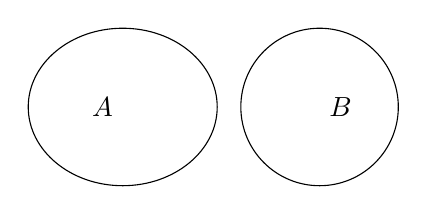
\begin{tikzpicture}[scale=1]
	\def\firstcircle{(0:0) ellipse (1.2 cm and 1 cm)}
	\def\secondcircle{(2.5,0) ellipse (1 cm and 1 cm)}
	\draw \firstcircle node[left]{$A$};
	\draw \secondcircle node [right]{$B$};
\end{tikzpicture}	}
\end{enumerate}

\subsubsection{CÔNG THỨC CỘNG XÁC SUẤT}


\begin{enumerate}[\iconMT]
	\item \indam{Công thức cộng xác suất:} Cho hai biến cố $A$ và $B$. Khi đó \boxmini{$\mathrm{P}(A \cup B) = \mathrm{P}(A) + \mathrm{P}(B) - \mathrm{P}(A \cap B)$}
	\item \indam{Đặt biệt:} Nếu hai biến cố $A$ và $B$ là xung khắc $\big(A \cap B = \varnothing\big)$ thì 
	\boxmini{$\mathrm{P}(A \cup B)=\mathrm{P}(A)+\mathrm{P}(B)$}
	\begin{luuy}
		Cho biến cố $A$ và biến cố đối $\overline{A}$. Ta có $\mathrm{P}(\overline{A})=1-\mathrm{P}(A)$.
	\end{luuy}
\end{enumerate}






